\chapter{Palier au manque de données sans augmentation artificielle des données}

\label{chapitre6}

\section{Motivation}

Dans ce dernier chapitre de contribution, nous allons détailler les nouvelles méthodes que nous avons appliqués à la reconnaissance d'émotions continues. Comme nous l'avons précédemment indiqué, le corpus AlloSat, quoique contenant 37 heures d'audio, n'est pas considéré comme un grand corpus, surtout si on parle uniquement de la partie utilisée pour l'apprentissage. En effet, les corpus utilisés pour l'apprentissage de système de reconnaissance sont plutôt de l'ordre de grandeur de la centaine d'heures. Cependant les architectures neuronales sont connues pour mieux fonctionner et mieux généraliser si elles sont apprises sur une grande quantité de données. Pour palier à ce problème, nous avons investi deux solutions différentes mais qui se sont révélées être complémentaires.

Tout d'abord, nous avons voulu bénéficier du contenu linguistique des conversations téléphoniques en complément du contenu acoustique.
En effet, ces informations sont déjà présentes implicitement dans les données d'entrée des différents systèmes, mais d'une part, elles ont été transformées, et d'autre part, il est possible que les modèles, n'ayant pas assez de données, n'aient pas réussi à dissocier les informations linguistiques des informations acoustiques. Nous avons donc fait le choix de traiter la modalité linguistique à part et de trouver la meilleure fusion permettant de profiter des caractéristiques présentes dans les deux modalités.

De plus, le pré-apprentissage permettant l'extraction de caractéristiques est une approche de plus en plus étudiée pour obtenir de meilleures représentations continues du contenu audio et textuel. Ces solutions ont pour but de compenser le manque de données sur une tâche courante en utilisant des données sur lesquelles sont appris des systèmes pour des tâches voisines. Ainsi, le travail d'apprentissage est facilité, puisqu'il ne part pas de zéro.

Enfin, nous avons combiné ces deux solutions, afin d'avoir des performances suffisantes permettant d'implémentater une nouvelle fonctionnalité de reconnaissance des émotions au sein des solutions logiciels de la société Allo-Média.

Ces différentes expérimentations et leurs résultats sont détaillées dans les sections suivantes. Mais avant cela, nous avons mis en place un score de confiance du score CCC. En effet, il est difficile d'analyser si un modèle est plus performant qu'un autre sans avoir mis en place un intervalle de confiance dans nos mesures.

\section{Confiance dans les scores CCC}
Comme nous l'avons expliqué précédemment, le score CCC est devenu un score de référence pour l'évaluation des systèmes de reconnaissance des émotions continues. %Cependant, nous n'avons pas trouvé d'intervalle de confiance ou de score de confiance associé à cette mesure.\textcolor{red}{ce n'est pas vrai=>
Cependant, nous n'avons pas trouvé d'expérience en reconnaissance des émotions continues  mentionnant l'utilisation d'un intervalle de confiance ou de score de confiance associé à cette mesure.

Nous avons donc cherché à mettre en place un intervalle de confiance. Notre travail se plaçant dans un contexte industriel, il est important de vérifier la pertinence des scores de nos modèles. En effet, comme notre corpus est assez petit, nous avons un nombre limité d'échantillons de test utilisés pour le calcul du score final.

%\textcolor{red}{attention pour cette section, c'est vraiment tu expliques comment fonctionne l'intervalle de confiance. Il manque des éléments comme par exemple ce qu'est la transformation de Fisher et pourquoi on l'utilise.}
En reprennant les travaux de Liao et al.~\cite{Liao2000} et McBride~\cite{McBride2005}, nous avons mis en place un intervalle de confiance du CCC. Nous repartons de la définition du CCC, présente dans l'équation~\ref{eq:CCC_rappel}.

\begin{equation}
   CCC = \frac{2\rho\sigma_x\sigma_y}{\sigma_x^2 + \sigma_y^2 + (\mu_x - \mu_y)^2}
\label{eq:CCC_rappel}
\end{equation}

Il s'agit d'un coefficient calculé entre deux vecteurs $x$ et $y$ à partir duquel on peut extraire :

\begin{itemize}
  \item l'écart type :
  \begin{equation}
      \sigma_x = \dfrac{1}{N} \sum_{i} \left(x_i - \mu_x\right)^2
  \end{equation}

  \item la covariance :
  \begin{equation}
    \sigma_{xy} = \dfrac{1}{N} \sum_{i} \left(x_i - \mu_x\right)\left(y_i - \mu_y\right)
  \end{equation}

  \item le coefficient de correlation :
  \begin{equation}
    \rho = \dfrac{\sigma_{xy}}{\sigma_{x} \sigma_{y} }
  \end{equation}
\end{itemize}

Afin d'avoir une meilleure approximation, on utilise la transformation de Fisher.
\textcolor{blue}{Cette transformation consiste à prendre la tangente hyperbolique inverse du coefficient de corrélation. Elle est utilisée pour palier aux cas où nous avons un coefficient de corrélation proche de ± 1, puisque dans ce cas sa distribution est fortement asymétrique, ce qui rend difficile l'estimation des intervalles de confiance pertinents. La transformation de Fisher résout ce problème en produisant une variable dont la distribution est approximativement distribuée normalement, avec une variance stable.} Comme dans les travaux de McBride, on appelle $\hat{Z}$ l'estimateur du CCC~\cite{McBride2005} défini dans l'équation~\ref{eq:hat_Z}

\begin{equation}
  \hat{Z} = \tanh^{-1}(\hat{\rho_c}) =  \dfrac{1}{2} \ln \left( \dfrac{1+ \hat{\rho_c} }{1 -\hat{\rho_c}}  \right)
  \label{eq:hat_Z}
\end{equation}

Nous pouvons calculer l'écart type de cet estimateur, en suivant l'équation~\ref{eq:et_hat_Z}.

\begin{equation}
\sigma_{\hat{Z} }^2 = \dfrac{\dfrac{(1-\rho^2) \hat{\rho_c} ^2}{(1-\hat{\rho_c}^2)\rho^2 } +  \dfrac{2\hat{\rho_c} ^3(1-\hat{\rho_c} )u^2}{\rho(1-\hat{\rho_c} ^2)^2} - \dfrac{\hat{\rho_c}^4 u^4}{2 \rho^2 (1-\hat{\rho_c}^2 )^2}}{N-2}
\label{eq:et_hat_Z}
\end{equation}

Avec un décalage effectué par rapport au paramètre d'échelle $u = \dfrac{\mu_x - \mu_y}{\sigma_x \sigma_y}$. \textcolor{blue}{j'avoue je ne sais pas pourquoi on fait cette opération.}

Ce qui nous permet de déduire un intervalle de confiance à $95\%$ pour le score de CCC selon l'équation~\ref{eq:inter_conf}.

\begin{equation}
    [\tanh (\hat{Z} - 1.64 \sigma_{\hat{Z}}); \tanh(\hat{Z} + 1.64 \sigma_{\hat{Z}})]
    \label{eq:inter_conf}
\end{equation}

Afin de se rendre compte de cet intervalle de confiance, nous avons donné quelques scores et leur intervalle associé dans le tableau~\ref{tab:inter_conf}.

\begin{table}
    \centering
    \begin{tabular}{|c|c|}
    \hline
         \textbf{Scores CCC} &\textbf{Intervalles de confiance associé} \\
         \hline
         0.7350	& [0.7324 ; 0.7375] \\
         0.7587	& [0.7563 ; 0.761] \\
         0.8054	& [0.8035 ; 0.8074] \\
         0.8524	& [0.8509 ; 0.854] \\
         0.8971	& [0.8960 ; 0.8982] \\
         \hline
    \end{tabular}
    \caption{Intervalles de confiance pour les scores CCC obtenus sur le sous-ensemble de Dev. Ils sont calculés sur différentes prédictions d'expérimentations sur l'initialisation des poids du réseau de neurones.}
    \label{tab:inter_conf}
\end{table}


Nous pouvons observer que l'intervalle de confiance est relativement faible. En effet, il ne concerne que les centièmes. De même que pour l'intervalle de confiance pour une variable aléatoire normale, on remarque également que plus le score est élevé, plus on a un faible intervalle. Par contre, on peut également constater que cet intervalle n'est pas symétrique.

Dans toutes les expériences suivantes, une différence de performance sera jugée significative uniquement si leur intervalle de confiance ne se chevauchent pas.

Un deuxième intervalle de confiance lié à l'initialisation peut également être calculé. Cet intervalle ne sera pertinent que dans le cas où l'on entraîne un nouveau modèle.

\section{Représentation linguistique}
Comme nous l'avons dit précédemment, la représentation linguistique peut apporter des informations qui diffèrent de celles retenues par les systèmes de la modalité acoustique. Pour mettre en place un système appris sur cette modalité, nous avons utilisé les transcriptions automatiques des conversations téléphoniques.

\subsection{Transcriptions automatiques}
Ces transcriptions sont obtenues à partir d'un système de reconnaissance de la parole utilisé dans l'entreprise Allo-Media issu des travaux de Rousseau et al.~\cite{Rousseau2014}. Le modèle acoustique est appris en utilisant le framework Kaldi~\cite{Povey2011} sur un volume d'environ mille heures de transcriptions manuelles de conversations issues de différents centre d'appels. Ainsi ce modèle est appris sur une grande quantité de données qualitatives, puisque manuelles mais aussi appropriées au domaine, puisque provenant de centre d'appels.

Le modèle linguistique appartient également à l'entreprise et il est mis à jour continuellement en utilisant les conversations transcrites automatiquement par l'entreprise. Chaque segment transcrit est associé à un score de vraisemblance, et seuls les segments ayant de haut scores sont utilisés pour remettre à jour le modèle linguistique.

Enfin le vocabulaire est également mis en place par l'entreprise, qui est partie d'un dictionnaire de français qu'un linguiste de l'équipe a phonétisé. Le vocabulaire a ensuite était manuellement vérifié pour retirer toute occurrence de mots n'ayant pas sa place dans des conversations de centre d'appels, afin de réduire les erreurs de reconnaissance dues à des mots à phonétique voisine ou aux homonymes. Ce travail est effectué de façon itérative en fonction des remontées des modérateurs. De plus, le vocabulaire est régulièrement mis à jour avec des noms de famille ou des noms de produits ou de marques.

\subsection{Synchroniser le linguistique et l'acoustique}
Comme notre objectif est d'utiliser conjointement la linguistique et l'acoustique, nous avons fait le choix de nous aligner sur les annotations émotionnelles dans les deux cas. Pour l'acoustique, nous extrayons un vecteur descripteur du signal toutes les 250~ms, soit un vecteur par pas d'annotation. Nous faisons la même chose pour le linguistique.

Pour cela, nous partons des CTM (\textit{time-marked conversation}) issus de la transcription automatique, comme par exemple ceux illustrés dans le tableau~\ref{fig:ctm}. Ce format se compose d'autant de lignes que de mots transcrits avec le code temps de l'émission du mot ainsi que la durée du mot. De plus, on peut retrouver à quel segment de parole sont associés tous les mots.

\begin{table}
    \centering
    \begin{tabular}{|l|l|l|l|l|l|l|}
      \hline
      Nom fichier &Canal &Début &Durée &Mot &\begin{tabular}[c]{@{}l@{}}Score \\
      Confiance \end{tabular} &id segment \\
      \hline
            ConvA &1 &5.23 &0.09 &oui &0.81 &ConvA-0000496-0001075 \\
            ConvA &1 &5.32 &0.27 &bonjour &1.00 &ConvA-0000496-0001075\\
            ConvA &1 &5.59 &0.36 &monsieur &1.00 &ConvA-0000496-0001075\\
            ConvA &1 &6.19 &0.27 &voilà &1.00 &ConvA-0000496-0001075\\
            ConvA &1 &6.46 &0.15 &j'ai &1.00 &ConvA-0000496-0001075\\
            ConvA &1 &6.61 &0.06 &un &1.00 &ConvA-0000496-0001075\\
            ConvA &1 &6.67 &0.39 &contrat &1.00 &ConvA-0000496-0001075\\
            ConvA &1 &7.06 &0.24 &chez &1.00 &ConvA-0000496-0001075\\
            ConvA &1 &7.30 &0.18 &vous &1.00 &ConvA-0000496-0001075\\
      \hline
    \end{tabular}
    \caption{Exemple de la transcription d'un début de conversation au format ctm mise sous la forme d'un tableau pour expliquer les différentes colonnes. Conversation issue du corpus AlloSat.}
\label{tab:ctm}
\end{table}



Nous définissons le protocole suivant pour aligner la transcription et l'annotation :
\begin{itemize}
  \item Tous les mots sont conservés, même les \textit{stop words}. Nous avons également fait des tests en supprimant ces mots tesl que définis dans le toolkit NLTK~\footnote{https://www.nltk.org/api/nltk.html}. Comme les performances finales de reconnaissance ne s'en retrouvaient pas améliorées, nous avons décidés de conserver tous les mots.
  \item Si un mot est prononcé dans plusieurs trames consécutives, le mot est dupliqué sur toutes les trames concernées.
  \item Si plusieurs mots sont prononcés dans la même trame, on conserve tous les mots prononcés. Pour les représenter, on fera la moyenne des représentations de chacun de ces mots.
\end{itemize}

Cette synchronisation nous permet de mettre l'acoustique et le linguistique sur le même plan, ce qui nous permettra par la suite d'utiliser conjointement les deux modalités pour la reconnaissance continue de la satisfaction et de la frustration.

\subsection{Exploration des word2vec}
Les plongements de mots, ou \textit{words embeddings} sont actuellement l'une des représentations continues les plus populaires de données textuelles. Ces plongements sont des représentations vectorielles appliquées à chacun des mots retrouvés dans le texte.
Parmi eux, word2vec~\cite{word2vec} est l'un des plus utilisés dans les tâches d'analyse des sentiments telles que la polarité ou la classification des états émotionnels~\cite{Dong2018}.

Afin de paramétrer des word2vec cohérents avec nos données, nous avons choisi d’entraîner nos propres représentations. Pour cela, nous avons entraîné un système avec le toolkit GENSIM~\cite{gensim}, en utilisant des données privées détenues par Allo-Media. Ces données sont composées de transcriptions manuelles d'appels reçues par les centres d'appels, totalisant plus de 4,5 millions de mots.

Deux algorithmes peuvent être utilisés pour apprendre ces représentations : \textit{CBOW} et \textit{skip-gram}, illustré dans la figure~\ref{fig:cbow_skip}. Pour \textit{CBOW}, le modèle prend en entrée les mots du contexte et prédit le mot cible en sortie. Pour \textit{skip-gram}, le modèle prend en entrée le mot cible et apprend à prédire les mots du contexte.

\begin{figure}[thb]
  \centering
    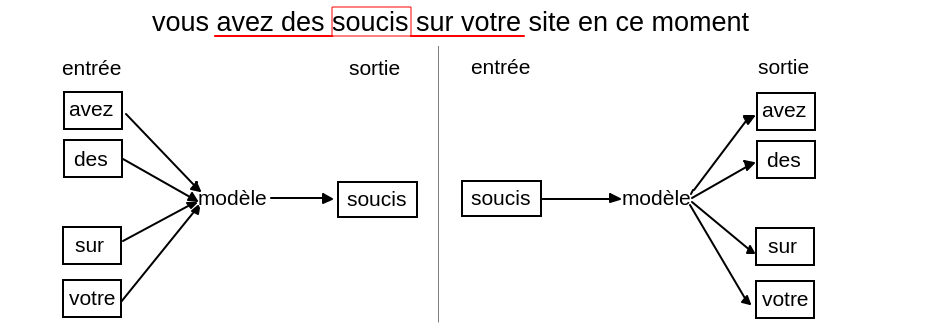
\includegraphics[width=14cm]{./Chapitre6/figures/cbow_skip.png}
    \caption{Représentation de l'apprentissage des word2vec selon deux algorithmes : le \textit{CBOW} (gauche) et le \textit{skip-gram} (droite). Ici on utilise un contexte de 5 mots, soit le mot cible entouré en rouge et deux mots de chaque coté, soulignés en rouge.
 %La partie gauche correspond à l'apprentissage avec \textit{CBOW} et la partie droite à l'apprentissage avec \textit{skip-gram}.
 }
    \label{fig:cbow_skip}
\end{figure}


Nous avons utilisé l'algorithme \textit{skip-gram} avec un contexte de 5 mots (soit le mot cible et 4 mots de contexte, 2 à gauche et 2 à droite). Le vocabulaire a été réalisé en incluant tous les mots présents dans le corpus. Tous les mots inconnus ont été remplacés lors de la transformation en une balise \textit{<UNK>} et ont donc tous la même représentation.

Afin de comparer les performances réalisées selon les différentes tailles de représentation utilisées, nous avons créé quatre ensembles de descripteurs, en faisant varier la taille des vecteurs:
\begin{itemize}
  \item \textbf{Word2vec-40} : La taille de la représentation a été fixée à 40 en raison des travaux préliminaires sur la modalité acoustique où nos représentations étaient de cet ordre de grandeur. Nous avons fait ce choix pour minimiser l'impact de la taille des descripteurs sur les performances du système,
  \item \textbf{Word2vec-100} : La taille des plongements est fixé à 100. Il s'agit d'une taille standard, beaucoup utilisée dans des tâches de NLP notamment.
  \item \textbf{Word2vec-150} : La taille des plongements est fixé à 150.
  \item \textbf{Word2vec-200} : La taille des plongements est fixé à 200. %Plus la taille des descripteurs est grande et plus on évite le sur-apprentissage généralement.
\end{itemize}

Nous avons utilisé l'architecture biLSTM-4 définie dans le chapitre~\ref{chapitre5} section~\ref{sec:5.3} pour tester la modalité linguistique représentée par des Word2vec. Les résultats sont disponibles dans le tableau~\ref{tab:res_word2vec}. Comme nous pouvons le remarquer, les scores sont supérieurs à 0.5 pour les quatre ensembles. Nous remarquons que les meilleurs scores sont atteints avec une taille de descripteurs de 100. Les performances se dégradent lorsque l'on a des tailles de descripteurs plus grandes.

Si nous comparons avec le maximum atteint par la modalité acoustique (cf section~\ref{sec:5.5.3}), soit 0.698 sur le dev et 0.513 sur le test sans post-traitement, nous voyons une amélioration de ce score maximum avec trois de nos ensembles. Avec un score CCC de 0.860 sur l'ensemble de développement et de 0.759 sur l'ensemble de test, la modalité linguistique représentée par des descripteurs Word2vec de taille 100 donne un résultat bien plus performant que tous les expérimentations effectuées sur la modalité acoustique seule.

\begin{table}[h]
  \centering
  \begin{tabular}{|l|l|l|}
  \hline
  Descripteurs   &Dev   &Test  \\
  \hline
  Word2vec-40    &0.805 &0.569 \\
  Word2vec-100   &\textbf{0.860} &\textbf{0.759} \\
  Word2vec-150   &0.592 &0.553 \\
  Word2vec-200   &0.668 &0.414 \\
  \hline
\end{tabular}
\caption{Score CCC des systèmes de reconnaissance des émotions d'une architecture neuronale bilstm à quatre couches en fonction des différents descripteurs d'entrée linguistiques.}
\label{tab:res_word2vec}
\end{table}

%\textcolor{red}{est-ce que le mauvais sscore obtenu avec word2vec-200 infirme la justification "limite le sur-apprentissage" ?}
Plusieurs justifications peuvent expliquer ce résultat. Tout d'abord, les mots sont porteurs d'informations émotionnelles qui sont moins souvent ambiguës que celles convoyées par la voix. On peut notamment mentionner les injures ou les mots contenus dans des champs lexicaux de polarité négative (par exemple ``inadmissible'', ``honteux'' ou encore ``arnaque'').

De plus, nous simplifions le travail du système de reconnaissance des émotions, puisque nous extrayons la modalité linguistique du signal audio et celle-ci est plus haut niveau. Lorsque l'on traite la modalité acoustique, les informations linguistiques sont toujours implicitement présentes et le système peut avoir des difficultés à les modéliser, notamment à cause du peu de données dont nous disposons.

De plus, les mots sont porteurs d'informations émotionnelles qui sont moins souvent ambiguës que celles convoyées par la voix. On peut notamment mentionner les injures ou les mots contenus dans des champs lexicaux de polarité négative (par exemple inadmissible, honteux ou encore arnaque).

Ces résultats nous permettent de valider l'utilisation de la modalité linguistique seule dans la détection de la satisfaction et de la frustration.

Nous avons donc chercher à tirer parti de ces deux modalités afin d'améliorer la reconnaissance de la satisfaction et de la frustration.

\section{Fusion des modalités acoustiques et linguistiques}
Comme nous l'avons défini dans le chapitre~\ref{chapitre3}, il existe plusieurs méthodes pour fusionner des modalités différentes. Chaque fusion a ses avantages et ses inconvénients et peut être plus ou moins adaptée aux descripteurs et aux modèles utilisés. Nous avons donc fait le choix de comparer les trois fusions existantes, à savoir la fusion des descripteurs, la fusion des modèles et la fusion de décision.

Ces trois fusions sont opérées sur les modalités acoustiques et linguistiques en utilisant le système biLSTM-4 précédemment introduit à la section~\ref{sec:5.3}. La figure~\ref{fig:archi_fusion} résume les quatre expérimentations dont nous rapportons les résultats dans le tableau~\ref{tab:res_fusion}.

\begin{figure}[thb]
  \centering
    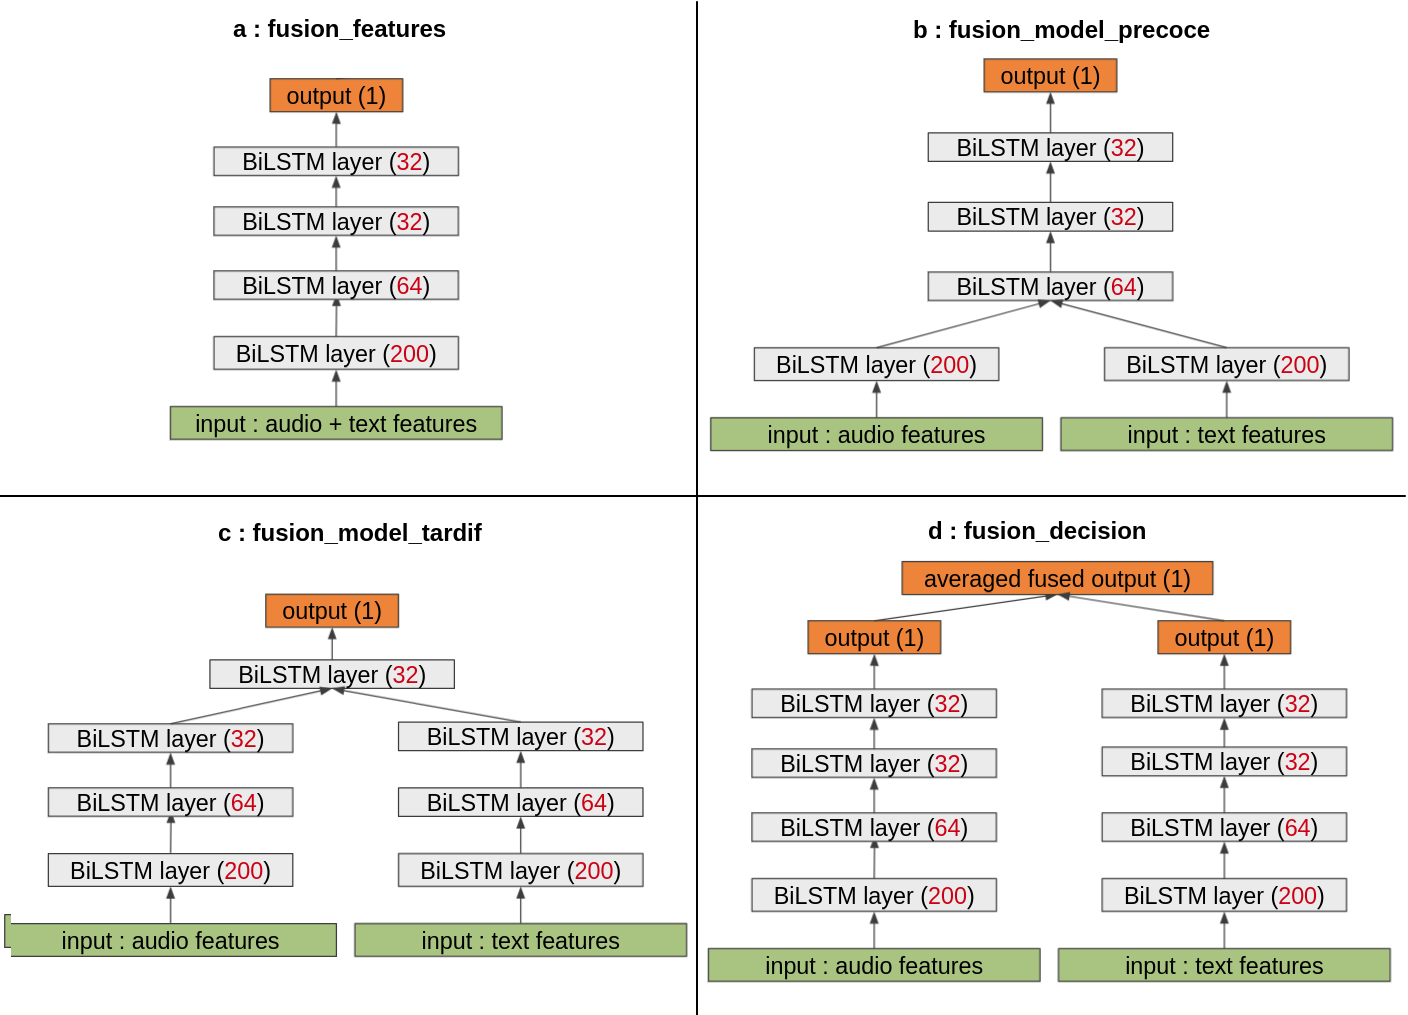
\includegraphics[width=18cm]{./Chapitre6/figures/archi_fusion.png}
    \caption{Représentation des quatre fusions utilisées pour la reconnaissance des émotions à partir des modalités acoustiques et linguistique. Les nombres entre parenthèses correspondent au nombre de neuronnes dans chaque couches.}
    \label{fig:archi_fusion}
\end{figure}


Les quatre architectures ont les caractéristiques suivantes:
\begin{itemize}
  \item \textbf{Fusion\_features} : La fusion s'effectue avant l'apprentissage en concaténant les descripteurs audio et texte. Une passe de normalisation est ensuite effectuée, pour ramener les descripteurs sur une même échelle. Il s'agit de la fusion la moins coûteuse, puisque nous n'avons qu'un seul modèle à entraîner, bien qu'il y ait plus d'entrées. Cette fusion correspond à la sous-figure a.
  \item \textbf{Fusion\_model\_precoce} : La fusion s'effectue  au niveau de la deuxième couche du réseau de neurone. Chaque modalité est d'abord traitée séparément dans la première couche, puis les deux sorties de ces deux couches sont concaténées avant d'être introduites dans la deuxième couche. La fusion précoce permet également de projeter les modalités dans des dimensions de même taille, sans pour autant que toutes les informations utiles soient déjà extraites avant d'être fusionnées. Cette fusion est modérément coûteuse, le nombre de paramètres lorsque les tailles des vecteurs d'entrée pour chaque modalité sont inférieures ou égales à 100, est du même ordre de grandeur que précédemment. Cette fusion correspond à la sous-figure b.
  \item \textbf{Fusion\_model\_tardif} : A l'inverse, la fusion va s'effectuer plus tard, au niveau de la quatrième couche du réseau. La sortie des troisièmes couches sont concaténées avant d'être données à la quatrième couche. Ce fusion tardive va prendre en compte des descripteurs très modifiés, desquels les informations importantes sont normalement déjà extraites. Cette fusion correspond à la sous-figure c.
  \item \textbf{Fusion\_decision} : Cette fusion s'effectue sur les sorties des deux modèles. On entraîne séparément deux modèles pour les deux modalités, puis on met en concours les deux vecteurs de sorties des deux modèles en utilisant une moyenne pondérée ou non. Cette fusion est la plus coûteuse puisque nous apprenons deux modèles distincts et que nous appliquons un post-traitement sur les sorties de ces modèles. Cette fusion correspond à la sous-figure d.
\end{itemize}

\begin{table}[h]
  \centering
  \begin{tabular}{|l|l|l|}
  \hline
  Descripteurs   &Dev   &Test  \\
  \hline
  \multicolumn{3}{|l|}{fusion features} \\
  \hline
  MFCC $\oplus$ word2vec-40        &.895  & .833 \\
  MFCC $\oplus$ word2vec-100        &.836  & .788 \\
  \hline
  \multicolumn{3}{|l|}{fusion modèle précoce} \\
  \hline
  MFCC-lib $\oplus$ word2vec-40       & .904 & .807 \\
  MFCC-lib $\oplus$ word2vec-100       & .829 & .797 \\
  \hline
  \multicolumn{3}{|l|}{fusion modèle tardive}   \\
  \hline
  MFCC-lib $\oplus$ word2vec-40    & .917  & .815  \\
  MFCC-lib $\oplus$ word2vec-100    & .881  & .717  \\
  \hline
  \multicolumn{3}{|l|}{fusion décision} \\
  \hline
  .66 Word2vec-40 + .34 MFCC-lib     &.897  &.840  \\
  .72 Word2vec-100 + .28 MFCC-lib    &.844 & .789 \\
  \hline
\end{tabular}
\caption{Comparaison des score CCC des systèmes de reconnaissance des émotions du biLSTM-4 en utilisant différent protocole de fusion et différents descripteurs pour la modalité linguistique.}
\label{tab:res_fusion}
\end{table}

Les résultats de ces différentes fusions sont disponibles dans le tableau~\ref{tab:res_fusion}. Nous observons que les scores de fusion, quelqu'ils soient, permettent d'égaler ou d'améliorer les résultats unimodaux. Nous remarquons que dans tous les types de fusion, c'est l'utilisation des word2vec-40 qui donne de meilleurs résultats. Cela peut être dû à la similarité entre les dimensions acoustiques et linguistiques : les MFCC-lib sont constitués de 48 descripteurs.
Nous pouvons également noter que le meilleur score atteint sur l'ensemble de dev ($0.917$) est attribué à la fusion tardive de modèle. Cependant, nous voyons que ce n'est pas la fusion de modèle qui donne le meilleur résultat sur l'ensemble de test. Le meilleur score ($0.840$) est atteint avec la fusion tardive. De plus l'écart entre le score de dev et de test est moins important pour la fusion tardive. Nous avons donc décidé de conserver la fusion tardive comme fusion de référence dans la suite de nos expérimentations.

Comme nous l'avons déjà présenté dans le chapitre~\ref{chapitre3}, les word2vec sont statiques : un mot a toujours la même représentation vectorielle, quel que soit le vrai sens du mot et le contexte de son apparition. Cela peut être problématique pour les mots polysémiques, par exemple fréquents en français~\cite{Pustejovsky1996}. C'est pour cette raison que nous avons souhaité mettre en place des représentations permettant de prendre en compte le contexte, que ce soit sur l'acoustique ou sur le linguistique.

\section{Descripteurs pré-entraînés}

L'apprentissage par transfert, \textit{transfert-learning} est largement utilisé dans l'analyse des sentiments, où de grandes bases de données non spécifiques sont utilisées pour former des caractéristiques génériques qui sont introduits dans le processus d’apprentissage.
Ce procédé permet de donner aux systèmes de meilleures capacités de généralisation compte tenu des données d'apprentissage fortement limitées~\cite{Dong2018}.

Une autre méthode permettant d'exploiter des modèles qui ont déjà vu une très grande quantité de données est d'utiliser des représentations auto-apprises. L'apprentissage auto-supervisé des représentations de la parole ou du langage a été proposé ces dernières années, par exemple avec le système BERT~\cite{Devlin2019}, utilisé pour la représentation textuelle que nous avons présenté au chapitre~\ref{chapitre2}.

De telles représentations, calculées par des modèles neuronaux entraînés sur d'énormes quantités de données non étiquetées, ont montré leur efficacité, par exemple pour la vision par ordinateur~\cite{Nanni2017} et des tâches de traitement du langage naturel (NLP) telles que de la
classification, de la similarité de texte, ou du classement par pertinence~\cite{Liu2019,Young2018,Yang2019}. Ils ont également prouvés leur efficacité dans les domaines de l'ASR~\cite{Kahn2020,Liu2020} et de la traduction~\cite{Nguyen2020}.

Néanmoins, ces représentations n'avaient jamais été utilisé pour de la reconnaissance d'émotions continues à notre connaissance. Nous avons donc proposé de tester cette approche pour réaliser notre tâche de reconnaissance des émotions. Il n'est, en effet, pas évident qu'elle soit pertinente pour la SER. Par exemple, au niveau acoustique, l'ASR a tendance à se concentrer sur des durées d'environ 30 ms, tandis que les émotions sont généralement prises en charge sur environ 1 seconde de parole.

Nous pensons que l'utilisation de ces représentations peut limiter l'impact du manque de données lorsque seules de petites bases de données sont disponibles pour former un réseau de neurones pour une tâche spécifique.

\subsection{Représentation linguistique}
Pour modéliser la partie linguistique, nous sommes partis sur des systèmes dérivés de BERT. Comme nous l'avons défini dans le chapitre~\ref{chapitre2}, BERT permet de donner une représentation contextuelle du texte. Il est cependant appris en majorité avec des occurrences anglaises. Comme nous voulons modéliser du français, nous nous sommes tournés vers CamemBERT~\cite{Martin2020} et FlauBERT~\cite{Le2020} que nous avons présenté également au chapitre~\ref{chapitre2}.

Chronologiquement, nous avons découvert CamemBERT en premier, et une fois que nous avions expérimenté avec ce modèle, nous avons comparé les résultats obtenus avec le modèle FlauBERT.

Pour l'extraction des descripteurs, nous avons utilisé le toolkit Fairseq~\cite{Ott2019}. Nous utilisons le modèle pré-entraîné, appelé \textit{camemBERT-base}, entraîné sur la partie française du corpus OSCAR~\cite{Ortizsuarez2019} constitué d'un ensemble de corpus monolingues extraits du \textit{Common Crawl snapshot} et totalisant 138Go de texte brut et 32,7 milliards de tokens après la tokenisation en sous-mots~\cite{Wu2016}. Les sous-mots sont des ensembles de caractères qui ne sont pas des mots à proprement parlé et qui sont déduit par le système de tokenisation, ici SentencePiece~\cite{Kudo2018}.

Les caractéristiques ont été extraites sur Allosat à l'aide de ce modèle pré-entraîné, et nous avons résumé les résultats au niveau du segment émotionnel (250~ms) en faisant la moyenne des représentations continues des sous-mots apparaissant dans le segment courant. Au total, nous utilisons un vecteur de caractéristiques à 768 dimensions.

Nous voulions également utiliser la variance de ces représentations, dans une volonté de comparer nos représentations aux précédentes qui utilisaient à la fois la moyenne et la variance des descripteurs. Cependant doubler le nombre de caractéristiques faisait exploser la complexité du réseau et donc le temps d'apprentissage.

Les résultats sont présentés dans le tableau~\ref{tab:res_camembert}. Comme nous pouvons l'observer, les modèles sont très performants pour la reconnaissance des émotions continues. Les descripteurs issus de CamemBERT donnent de meilleurs résultats que ceux issus de FlauBERT même s'ils restent du même ordre de grandeur. Si on se compare aux meilleurs résultats des word2vec, à savoir respectivement $0.860$ et $0.759$ sur le dev et le test, on obtient une amélioration du score CCC de 0$.036$ sur le dev et de $0.040$ sur le test.

\begin{table}[h]
  \centering
  \begin{tabular}{|l|l|l|}
  \hline
  Descripteurs   &Dev   &Test  \\
  \hline
  CamemBERT      &\textbf{0.896} &\textbf{0.799} \\
  FlauBERT       &0.874 &0.733 \\
  \hline
\end{tabular}
\caption{Scores CCC des systèmes de reconnaissance des émotions du biLSTM-4 en prenant en entrée des descripteurs linguistiques pré-entrainés.}
\label{tab:res_camembert}
\end{table}


\subsection{Représentation acoustique}
Dans le domaine du SER, trouver le meilleur ensemble de caractéristiques acoustiques est toujours un sous-domaine de recherche actif~\cite{Jing2018}.

Comme nous l'avons déjà dit (cf section~\ref{sec:3.3.1}), la plupart des ensembles de caractéristiques \textit{experts}~\cite{Eyben2016,Schuller2013} visent à décrire la prosodie dans le signal, avec des descripteurs de bas niveau (LLD) capturant l'intensité, l'intonation, le rythme ou la qualité de la voix.
Une autre approche consiste à extraire des caractéristiques spectrales : les coefficients cepstraux à fréquence mel (MFCC) sont clairement les plus utilisés car ils sont robustes aux signaux bruités même s'ils n'ont pas été conçus pour la prosodie ou l'émotion.

Récemment, wav2vec~\cite{Schneider2019} et Audio AlBERT~\cite{Chi2020} ont été introduits dans les domaines de la reconnaissance automatique de la parole et dans l'identification du locuteur comme l'une des premières approches pré-entraînées pour extraire des caractéristiques contextuelles des signaux bruts.
Comme nous l'avons expliqué au chapitre~\ref{chapitre2}, wav2vec~\cite{Schneider2019} est un modèle pré-entraîné par auto-supervision : il apprend à prédire les futurs échantillons à partir de l'une analyse de le fenêtre courante.

Dans nos expérimentations, nous utilisons deux modèles pré-entraînés. Le premier, appelé \textit{wav2vec-EN}, fourni par Schneider et al.,  a été entraîné sur le corpus Librispeech~\cite{librispeech} qui est composé de 960 heures de livre audio en anglais.
Nous formons également notre propre modèle, appelé \textit{wav2vec-FR}, dérivé du premier modèle et fine-tuné sur les conversations non étiquetées de centres d'appels français correspondant à plus de 500 heures de données privées.

Comme ce modèle est appris avec des audios échantillonnés à 16kHz, nous avons sur-échantillonné nos données pour qu'elles correspondent aux modèles. Nous avons utilisé la fonction de rééchantillonnage FFMpeg~\cite{Tomar2006} avec la fonction d'interpolation \textit{sinc}.

Au final, chaque segment émotionnel est représenté par un vecteur de taille 512 qui se compose des valeurs moyennes des plongements obtenus toutes les 10~ms sur le segment émotionnel, \textit{i.e.} soit une moyenne de 25 valeurs pour AlloSat. Comme pour la représentation linguistique, nous avons uniquement conservé la moyenne et non l'écart type pour de pas avoir des vecteurs d'entrée trop important qui aurait fait exploser la complexité et donc le temps d'apprentissage et les ressources nécessaires pour le mener à bien.

\begin{table}[h]
  \centering
  \begin{tabular}{|l|l|l|}
  \hline
  Descripteurs   &Dev   &Test  \\
  \hline
  wav2vec-EN      &0.851 &\textbf{0.730} \\
  wav2vec-FR      &\textbf{0.865} &0.635 \\
  \hline
\end{tabular}
\caption{Score CCC des systèmes de reconnaissance des émotions du biLSTM-4 en prenant en entrée des descripteurs acoustiques pré-entrainés.}
\label{tab:res_wav2vec}
\end{table}


Les résultats sont présentés dans le tableau~\ref{tab:res_wav2vec}. Comme nous pouvons l'observer, les modèles sont également très performants pour la reconnaissance des émotions continues. Les descripteurs issus de wav2vec-EN donne de meilleurs résultats que ceux issus de wav2vec-FR même s'il reste dans la même ordre de grandeur. Cela peut être expliqué par le fine-tuning effectué sur à peine 500 heures de données, ce qui a pu suffisamment dérégler le modèle sans pour autant lui faire intégrer des renseignements pertinents. Si on se compare aux meilleurs résultats des MFCCs, à savoir respectivement $0.698$ et $0.513$ sur le dev et le test, on peut affirmer que la représentation wav2vec-EN permet au système de mieux reconnaître les états émotionnels, puisqu'on améliore les scores respectivement de $0.153$ et $0.217$ sur le dev et le test.

\subsection{Reproduction sur SEWA}
Afin d'étendre l'utilisation des descripteurs pré-entraînés, nous avons voulu tester les performances d'un système biLSTM-4 apprenant avec ce type de descripteurs pour le corpus SEWA. Le corpus étant en allemand et en hongrois, nous avons uniquement considéré le modèle wav2vec-EN.

\begin{table}[h]
  \centering
  \begin{tabular}{|l|l|l|l|}
  \hline
  Descripteurs   &Activation   &Valence  &Liking  \\
  \hline
  wav2vec-EN      &0.251      &0.215      &0.254 \\
  \hline
\end{tabular}
\caption{Scores CCC des systèmes de reconnaissance des émotions du biLSTM-4 en prenant en entrée des descripteurs acoustiques pré-entrainés sur l'ensemble de dev du corpus SEWA.}
\label{tab:sewa_wav2vec}
\end{table}


Les résultats sont présentés dans le tableau~\ref{tab:sewa_wav2vec}. Les scores obtenus sur les dimensions de l'activation et de la valence sont moins élevés que lorsque l'on utilise les ensembles de descripteurs MFCCs ou eGeMAPS. Cependant on peut constater une amélioration sur l'axe du liking, mais qui n'atteint pas un score suffisant pour être considéré comme une réussite.

Dans le cas du corpus SEWA, l'utilisation de descripteurs pré-entraînés ne semble pas permettre d'améliorer les performances du système. Notre hypothèse réside dans la différence de quantité de données entre les deux corpus : le set de train d'AlloSat est composé de 25 heures d'enregistrement audio alors que celui de SEWA a moins de 2 heures de conversations. %Malgré l'utilisation des descripteurs pré-entraînés, le réseau n'est pas en mesure d'obtenir de bons résultats, probablement en raison de la faible quantité de données.
Nous pensons également que la conception du corpus SEWA peut avoir un impact sur la performance de ces descripteurs. Le fait que SEWA soit composé de conversations dyadiques où deux locuteurs sont présents dans le même document peut complexifier le processus d'extraction de descripteurs, alors qu'AlloSat ne contient que la voix du client.

Nous avons vu précédemment que la fusion des deux modalités, en considérant les descripteurs MFCC et word2vec, permet d'améliorer les performances du système. Nous expérimentons donc la fusion des descripteurs pré-appris.

\section{Fusion des modalités acoustiques et linguistiques pré-entraînés}
Différents protocoles de fusion ont été explorés : fusion features (concaténation des vecteurs wav2vec et camemBERT), fusion au niveau du modèle (au niveau de la première et de la dernière couche) et fusion de décision. Les fusions features et au niveau du modèle requièrent beaucoup plus de temps d'apprentissage, puisque nous doublons le nombre d'entrées du réseau (768+512). De plus, les résultats que nous avons obtenus sur ces features sont peu intéressants puisqu'au niveau des scores d'unimodalité. Nous ne les présentons pas dans ce document.

Comme jusqu'à présent la modalité linguistique donne de meilleurs résultats que la modalité acoustique et que la dimension des descripteurs camemBERT est grande, nous avons voulu quantifier l'apport de ces descripteurs en les comparant aux descripteurs word2vec. Ainsi en fonction de l'ordre de grandeur de cet apport, nous pourrons statuer sur la pertinence ou non de l'utilisation de plus de ressources.

\begin{table}[h]
  \centering
  \begin{tabular}{|l|l|l|l|}
  \hline
  Descripteurs &nombre features   &Dev   &Test  \\
  \hline
  %\multicolumn{4}{|l|}{fusion décision} \\
  %\hline
  .66 word2vec-40 + .34 MFCC-lib     &47 + 40 &0.897  &0.840  \\
  .63 wav2vec-EN + .37 word2vec      &512 + 40 &0.878 &0.750 \\
  .28 wav2vec-EN + .72 CamemBERT        &512 + 768 &\textbf{0.932} &\textbf{0.920} \\
  %.31 wav2vec-EN + .69 camemBERT     &512 + 768 &\textbf{0.907}   &\textbf{0.825} \\
  \hline
\end{tabular}
\caption{Comparaison des score CCC des systèmes de reconnaissance des émotions du biLSTM-4 en utilisant la fusion de décision avec des descripteurs pré-entrainés. Nous rappelons les scores obtenus précédemment avec la fusion des descripteurs baseline.}
\label{tab:res_fusion_pretrain}
\end{table}


Comme pour les résultats précédents sur la fusion des descripteurs de la baseline (MFCC + word2vec), la fusion de décision permet d'améliorer les résultats même si l'amélioration est moins forte que précédemment. Comme nous le rapportons dans le tableau~\ref{tab:res_fusion_pretrain}, nous atteignons des scores de $0.932$ sur le dev et $0.920$ sur le test, ce qui correspond à une augmentation significative des scores. On remarque également que la fusion des ensembles wav2vec-EN et word2vec donne de moins bons résultats, et que c'est la modalité acoustique qui prime dans cette fusion. On peut supposer que la trop grosse différence dans le type de descripteur ne va pas permettre une bonne fusion.

Nous atteignons donc des scores très performants pour la reconnaissance des émotions continues sur le corpus AlloSat, permettant à l'entreprise de penser à la commercialisation de cet indicateur.

\section{Conclusion}
Dans ce chapitre, nous avons décrit les différents choix que nous avons considéré pour améliorer nos performances en terme de reconnaissance continue des émotions. Après une discussion autour de la confiance dans les scores CCC, nous avons mis en place une représentation linguistique des conversations que nous avons fusionné avec la représentation acoustique. De plus, nous avons mis en place des nouveaux modèles entraînés avec des descripteurs pré-entraînés.

Nous pouvons conclure que le meilleur système de reconnaissance des émotions continues utilise un réseau de neurones récurrents, une utilisation des deux modalités en les fusionnant et des entrées issues de descripteurs pré-entraînés.

Ces scores a l'état de l'art sont très corrects, mais une question reste en suspens : pourquoi la modalité linguistique permet une telle amélioration de la reconnaissance continue des émotions ? Nous allons tenter de répondre à cette question dans le prochain chapitre.
